\section{Android Application for SSPS Demo} \label{android}

The Android application has the role of subscriber. There are three publishers; each one is a separate Java client. Another important entity, the Sampling Broker is running alongside a Moquette broker as a part of it.

\subsection{Setup}

\subsubsection{Publishers and Sampling Broker}

The publishers and the Sampling Broker are running on a server with the following configuration:

\begin{itemize}
    \item \textbf{System:} VMware Virtual Platform
    \item \textbf{CPU:} 2 X Intel(R) Xeon(R) CPU X5650  @ 2.67GHz
    \item \textbf{Memory:} 3004 MiB
    \item \textbf{OS:} Ubuntu SMP
\end{itemize}

\subsubsection{Android application}

To demo the SSPS, we limit the bandwidth connection on the Android device to 10KB/s using the application \textit{BradyBound} \parencite{brady}. The Android application itself is running on a device with the following configuration:

\begin{itemize}
    \item \textbf{Android Device:} Hisense Sero 7 Pro
    \item \textbf{CPU:} 1.2GHz Nvidia Tegra 3
    \item \textbf{Memory:} 1 GB
    \item \textbf{OS:} Android 6.0
\end{itemize}

\subsection{Result}

Once connected to the broker, we can receive notifications in different formats(XML, CSV, and JSON) and different types(compressed and uncompressed) depending on the subscription.

Figures \ref{figures:xml_u} and \ref{figures:xml_c} shows the throughput for uncompressed notifications (without SSPS) and compressed notifications (with SSPS) for the XML data type respectively. The increase in throughput from \textasciitilde17 notifications/sec to \textasciitilde55 notifications/sec clearly shows the advantage of using the SSPS for mobile applications.

Similar results can be seen for CSV data format in Figures \ref{figures:csv_u} and \ref{figures:csv_c} with a throughput of \textasciitilde60 notifications/sec in case of uncompressed notifications and \textasciitilde125 notifications/sec in case of compressed notifications. 

Further, same result is also seen in case of JSON data format in Figures \ref{figures:json_u} and \ref{figures:json_c} with a throughput of \textasciitilde23 notifications/sec in case of uncompressed notifications and \textasciitilde65 notifications/sec in case of compressed notifications.

\makeatletter
\setlength{\intextsep}{20pt}
\makeatother

\begin{figure}[h!]
\centering
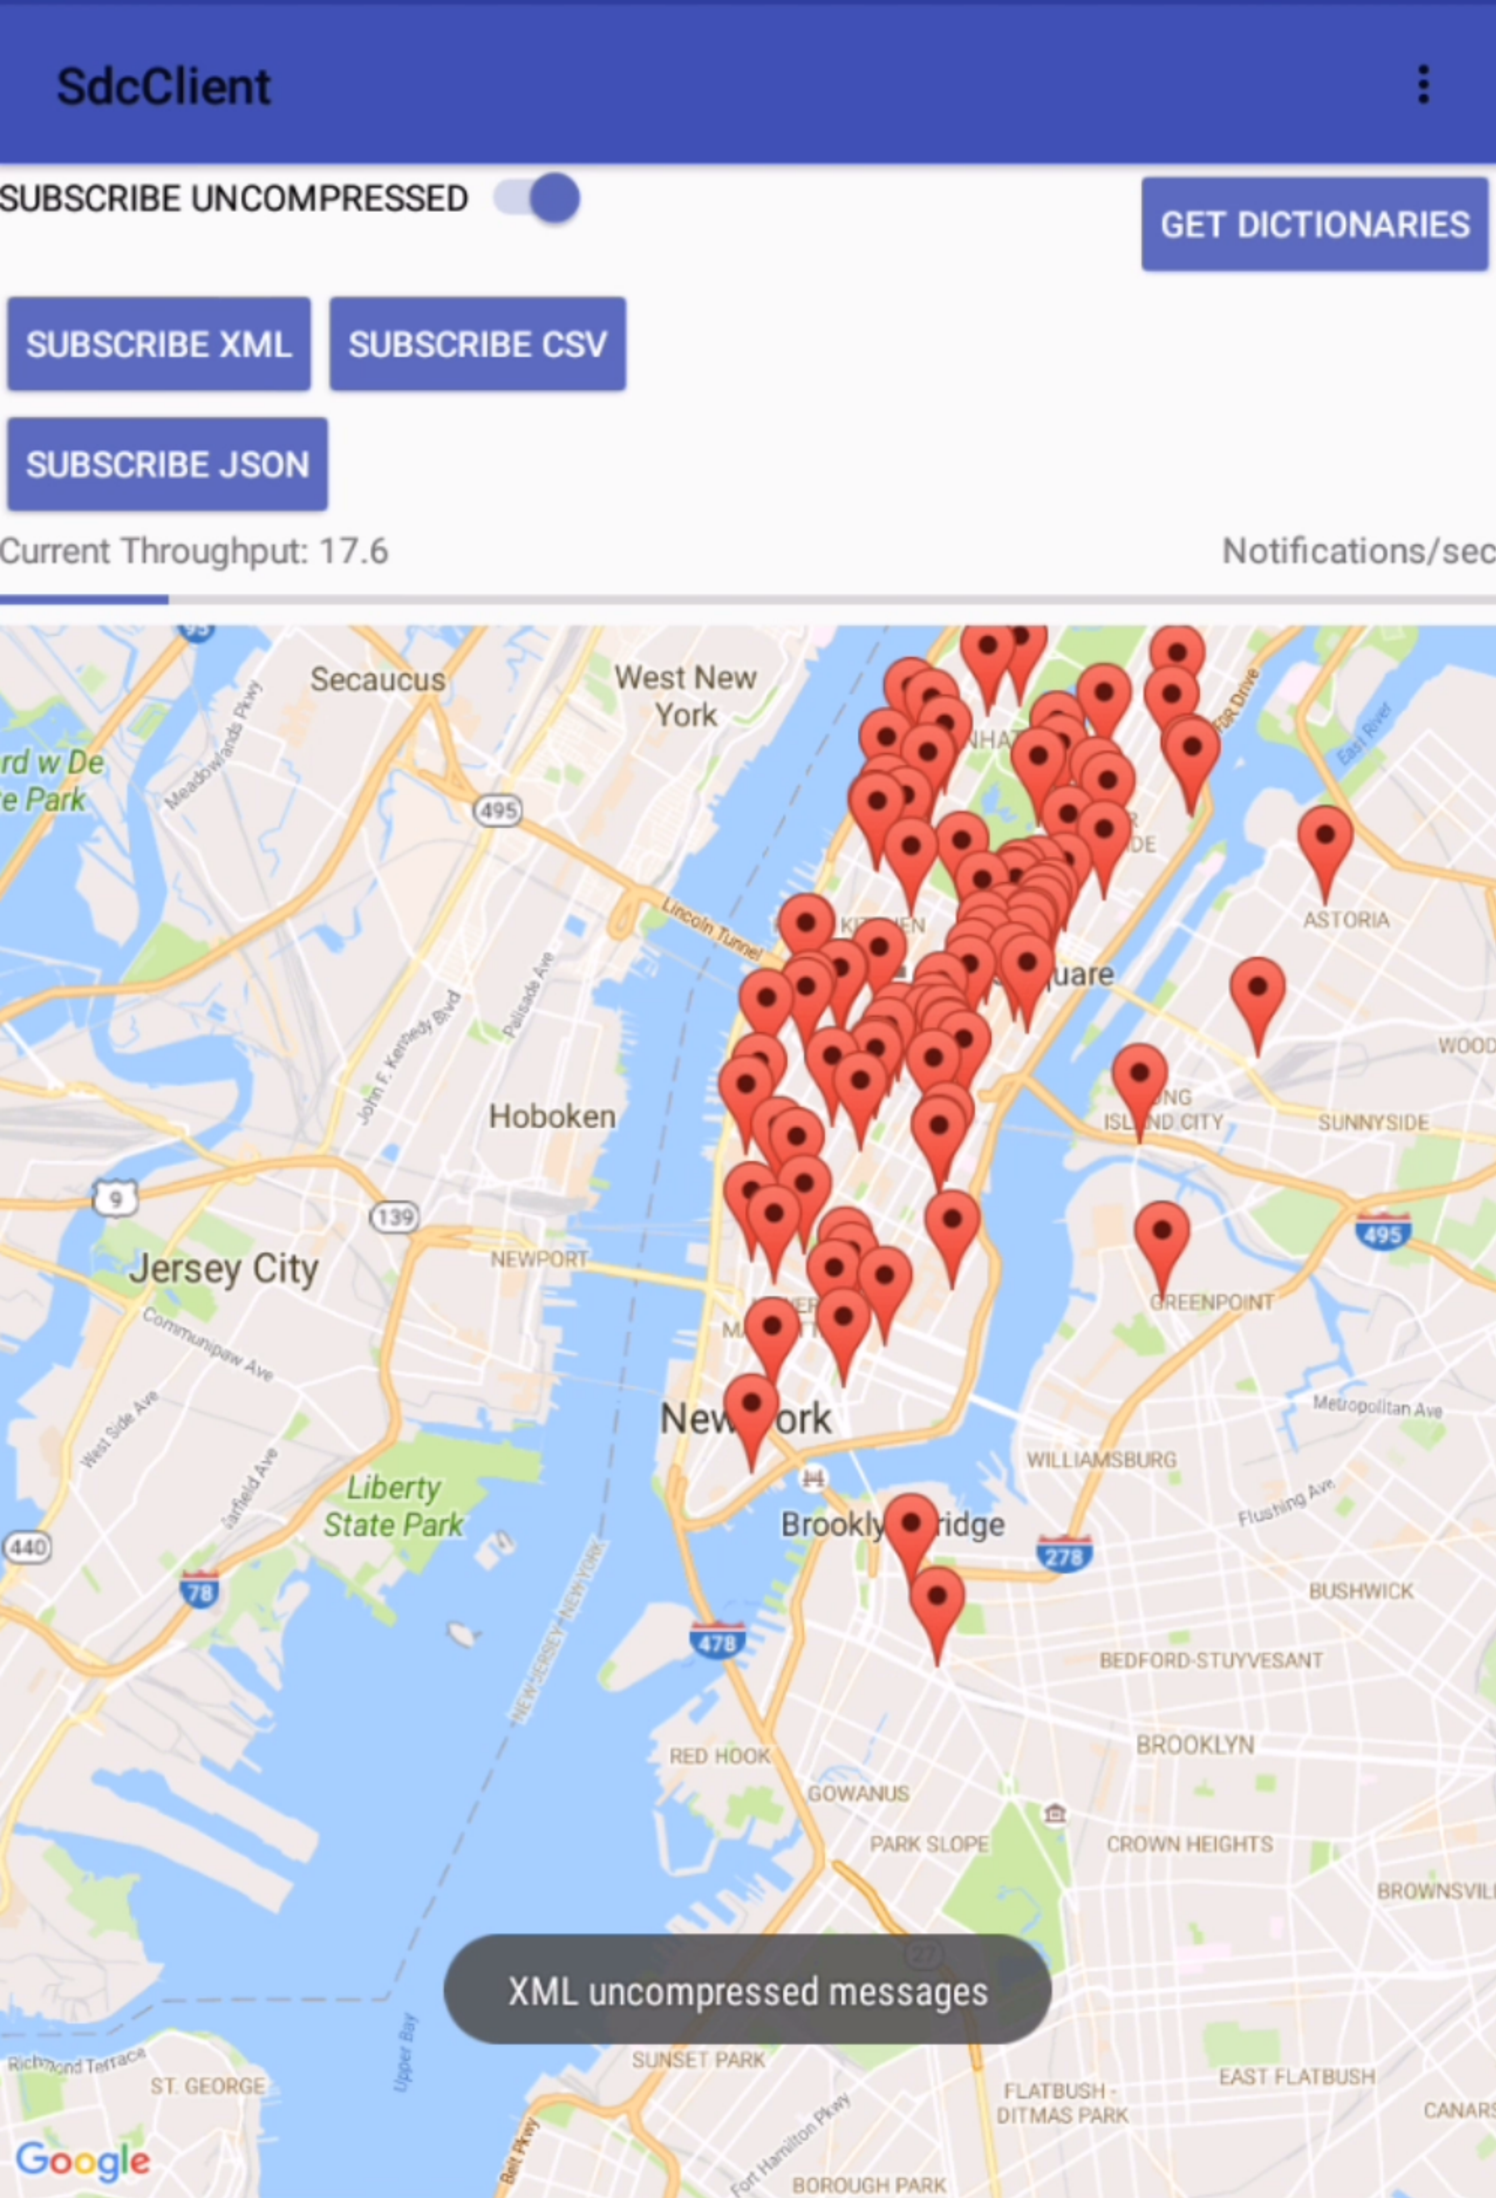
\includegraphics[scale=0.5]{xml_u.pdf}
\caption{XML uncompressed notifications}\label{figures:xml_u}
\end{figure}


\begin{figure}[h!]
\centering
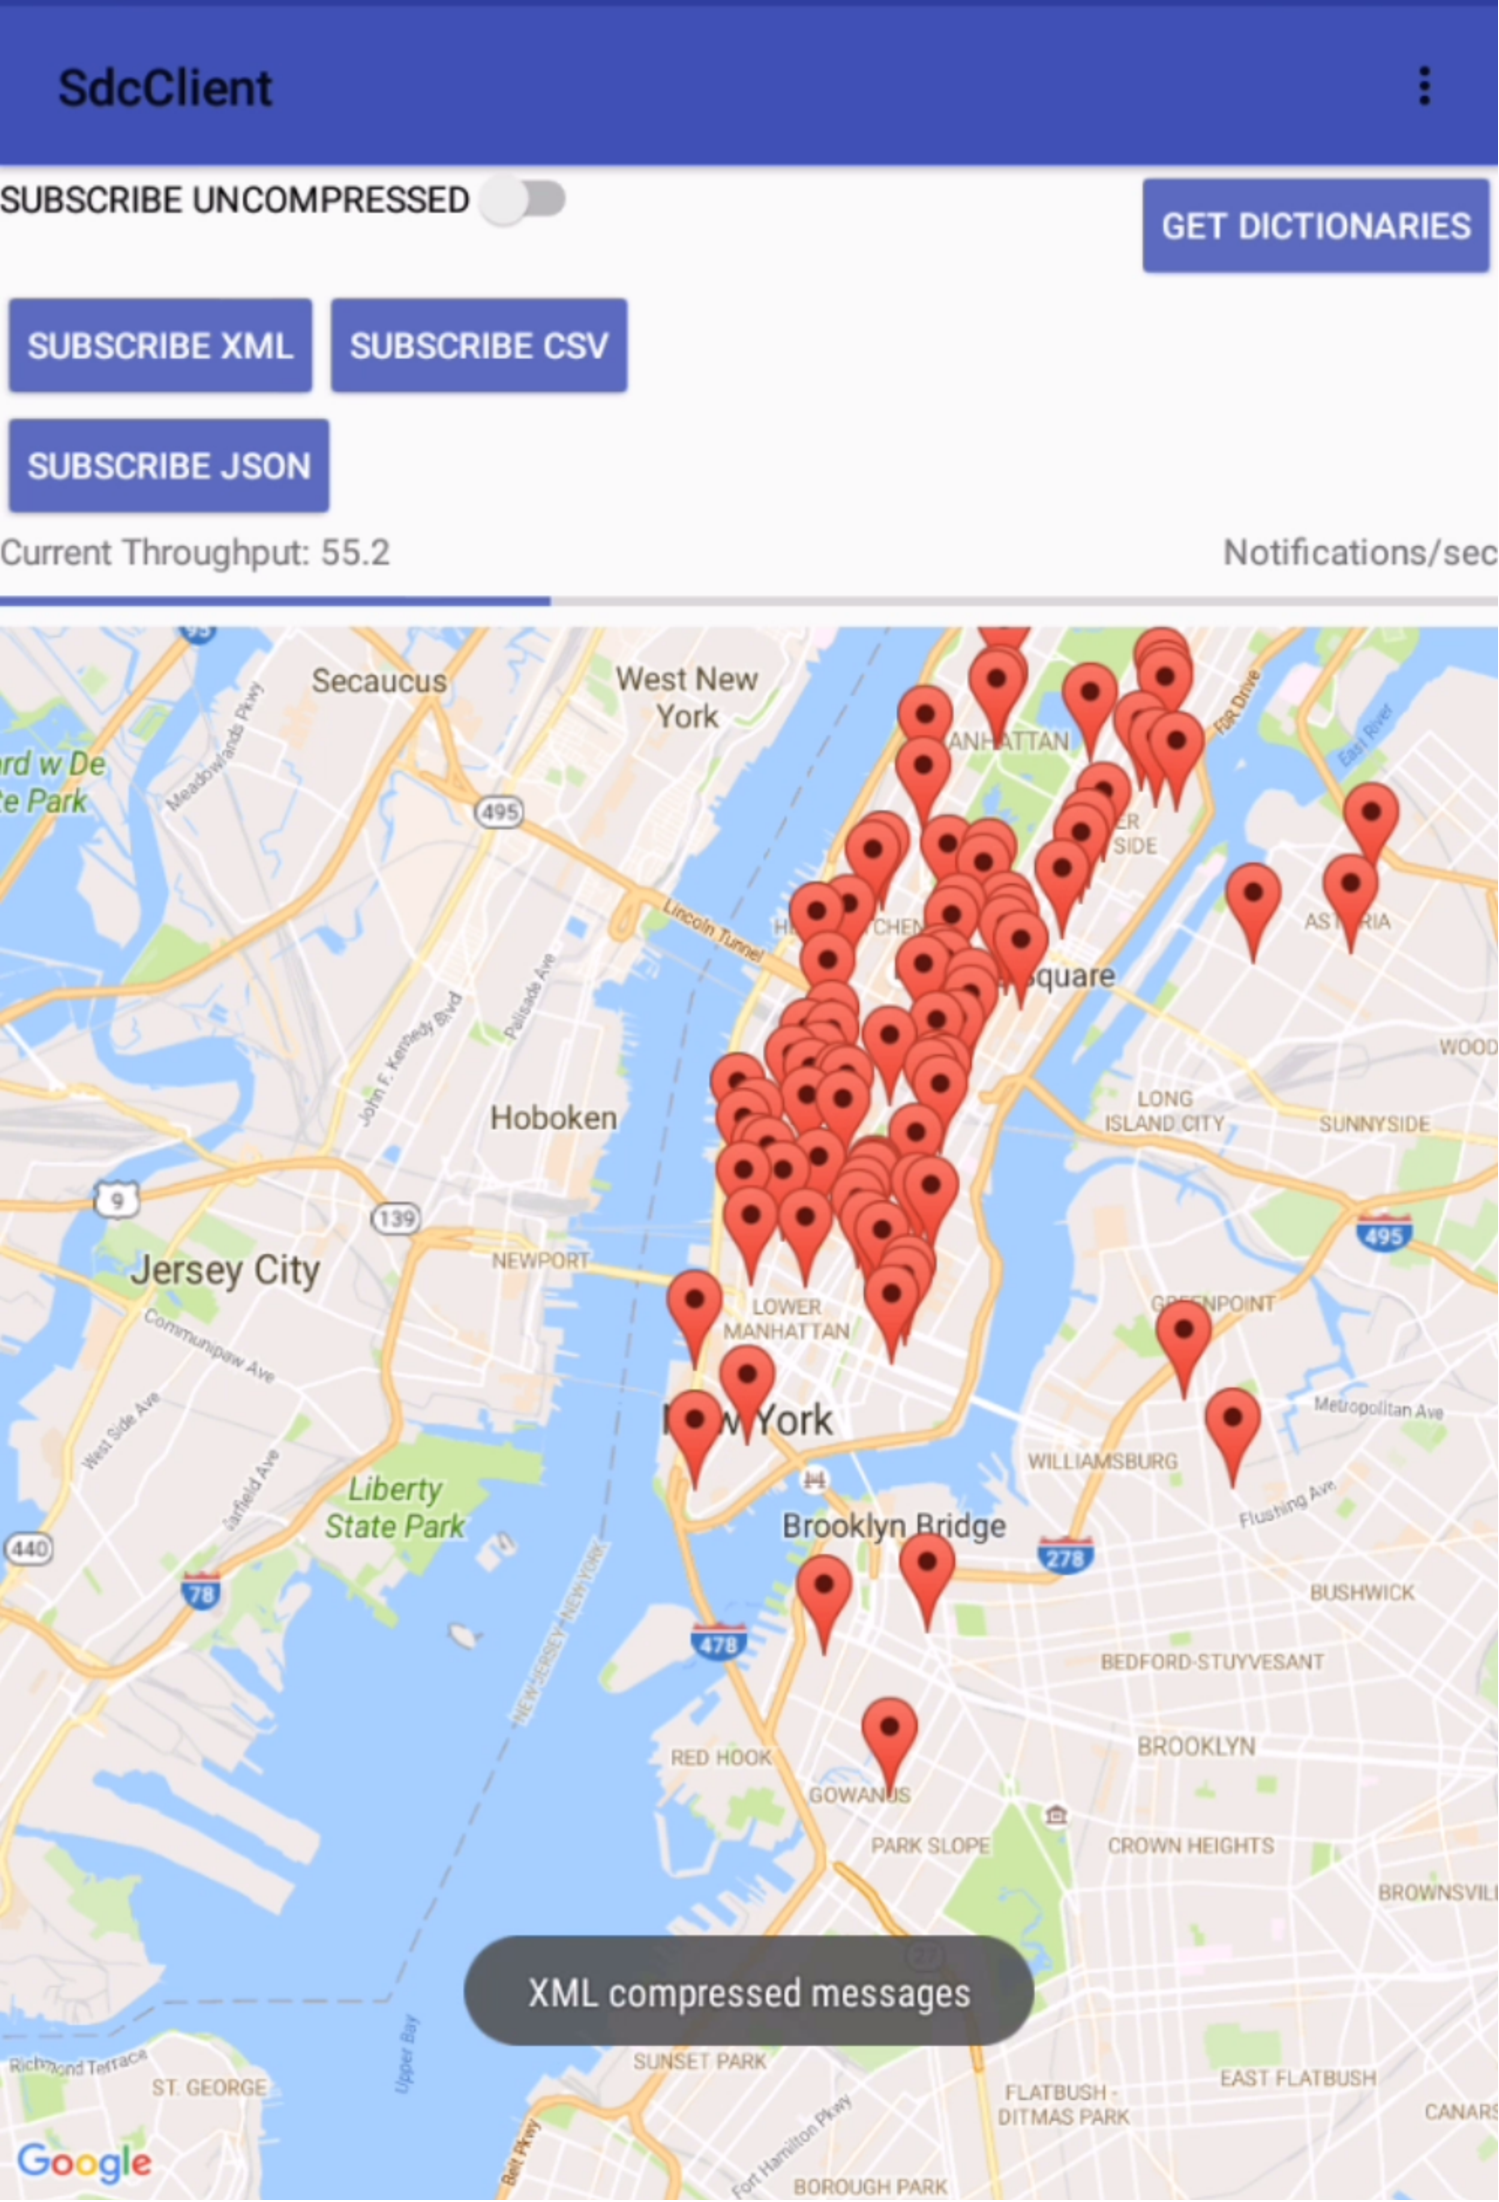
\includegraphics[scale=0.5]{xml_c.pdf}
\caption{XML compressed notifications}\label{figures:xml_c}
\end{figure}

%%%%%%%%json%%%%%%

\makeatletter
\setlength{\@fptop}{0pt plus 1fil}
\setlength{\@fpbot}{0pt plus 1fil}
\makeatother

\begin{figure}
\noindent\begin{minipage}{.5\textwidth}
  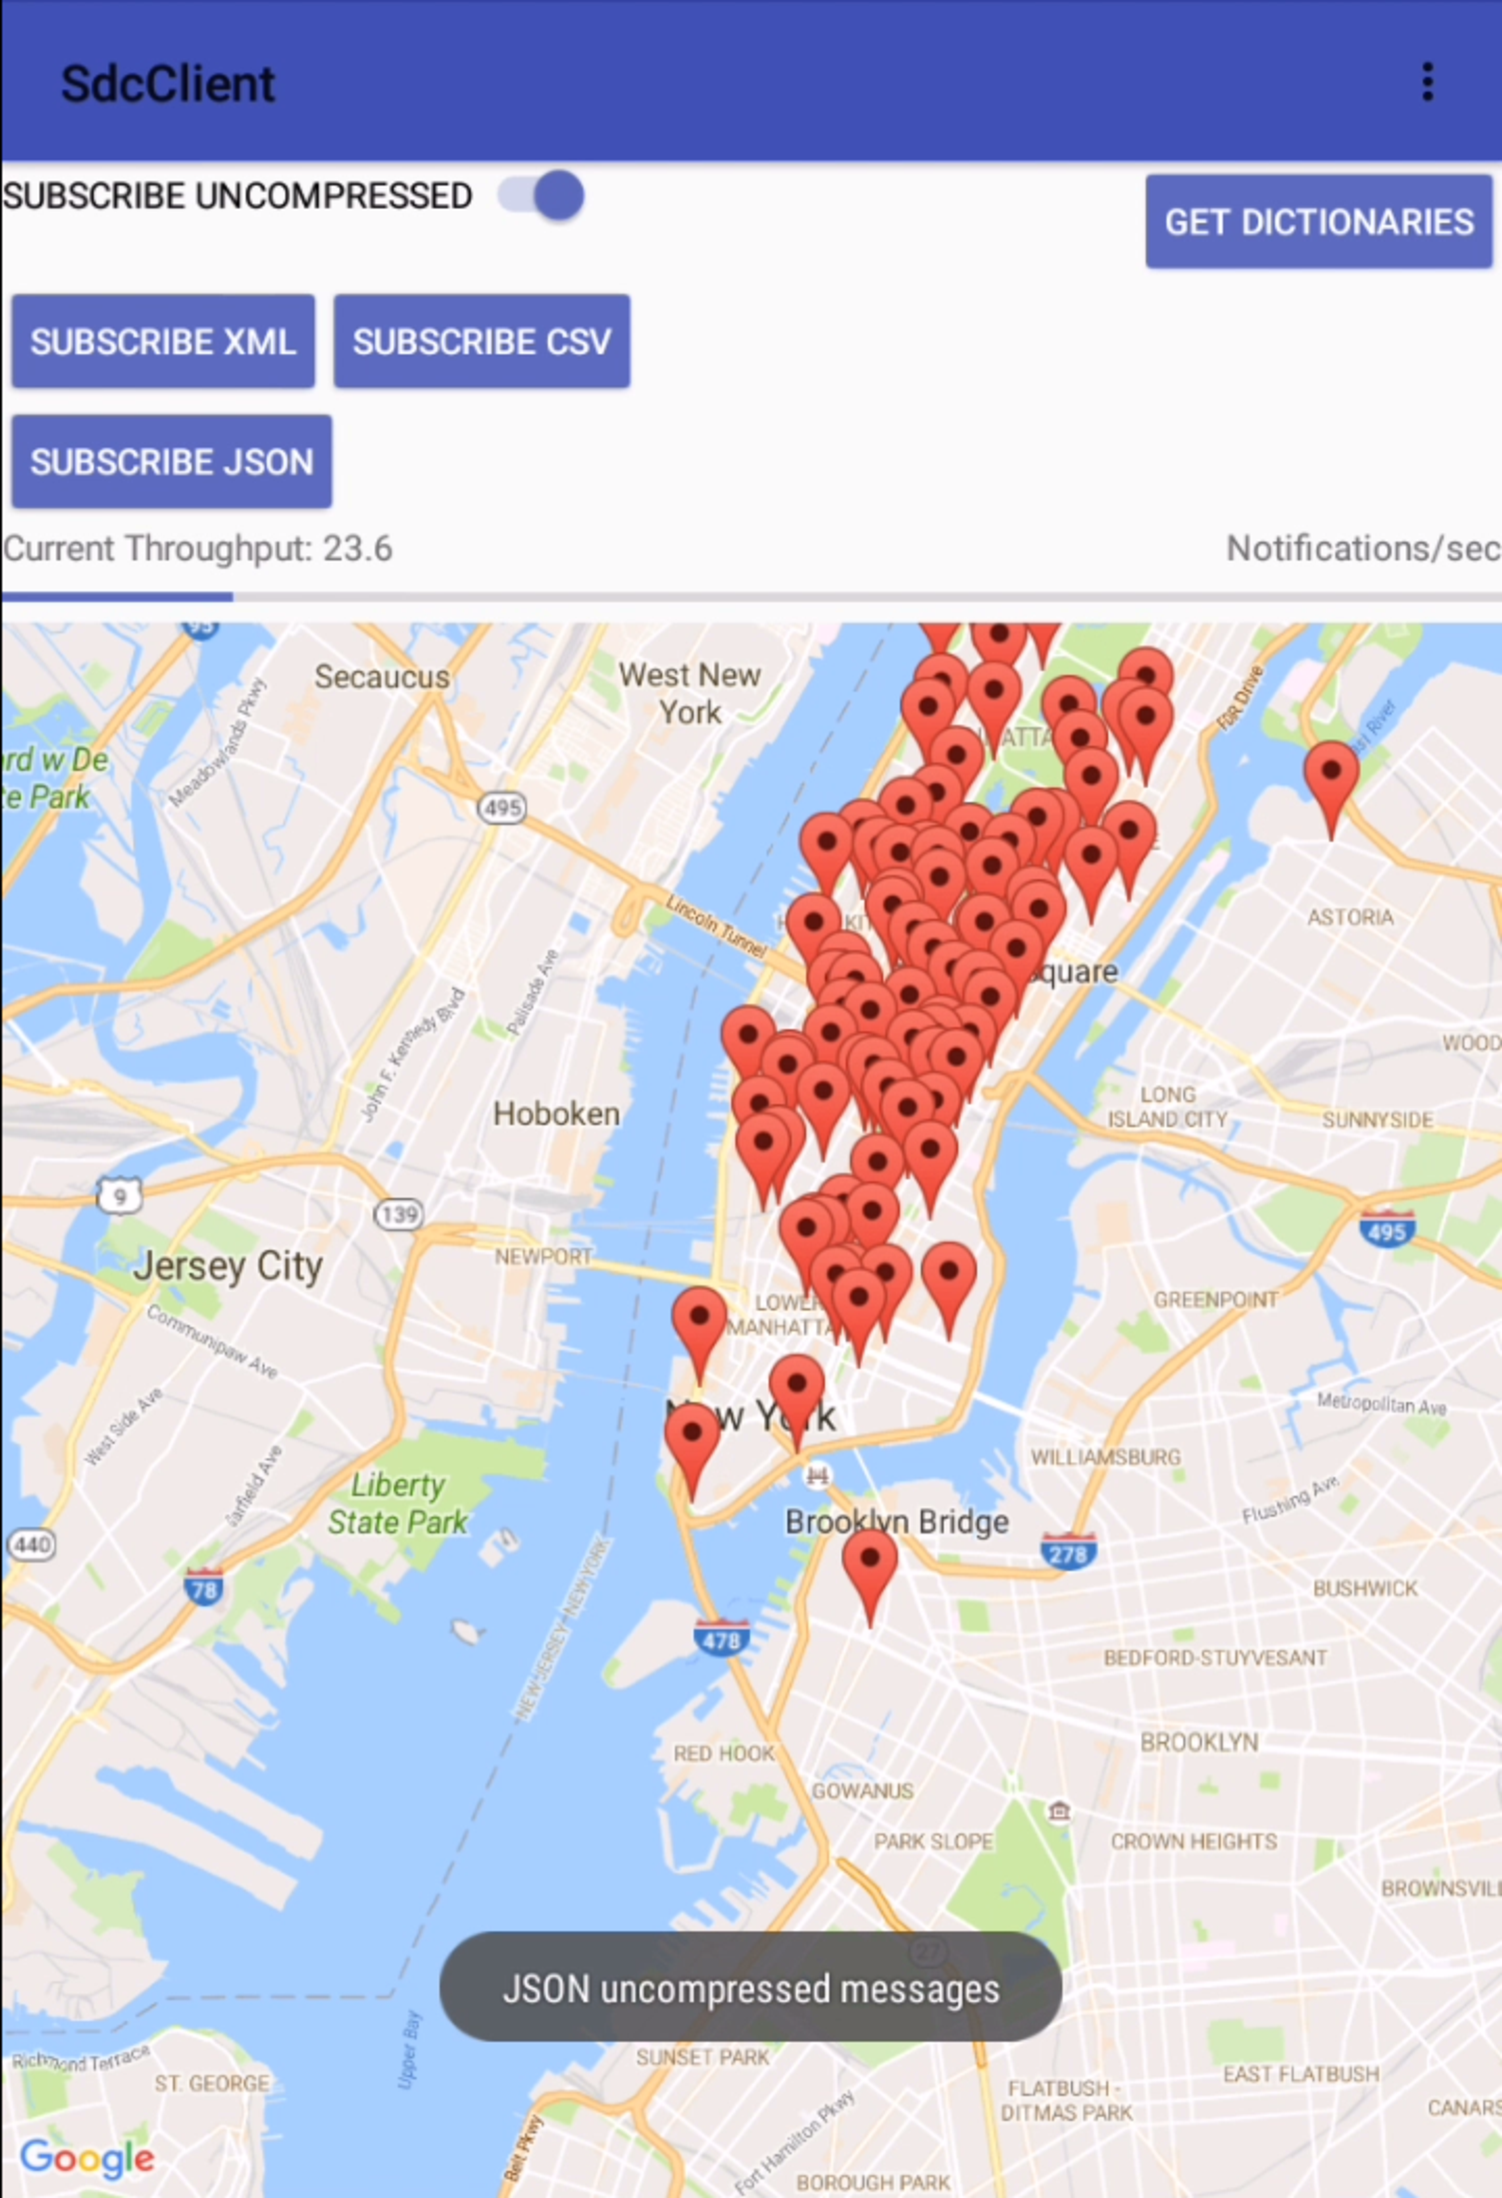
\includegraphics[scale=0.28]{json_u.pdf}
  \captionsetup{width=0.9\textwidth}
  \caption{JSON~uncompressed notifications}
  \label{figures:json_u}
\end{minipage}%
\noindent\begin{minipage}{.5\textwidth}
  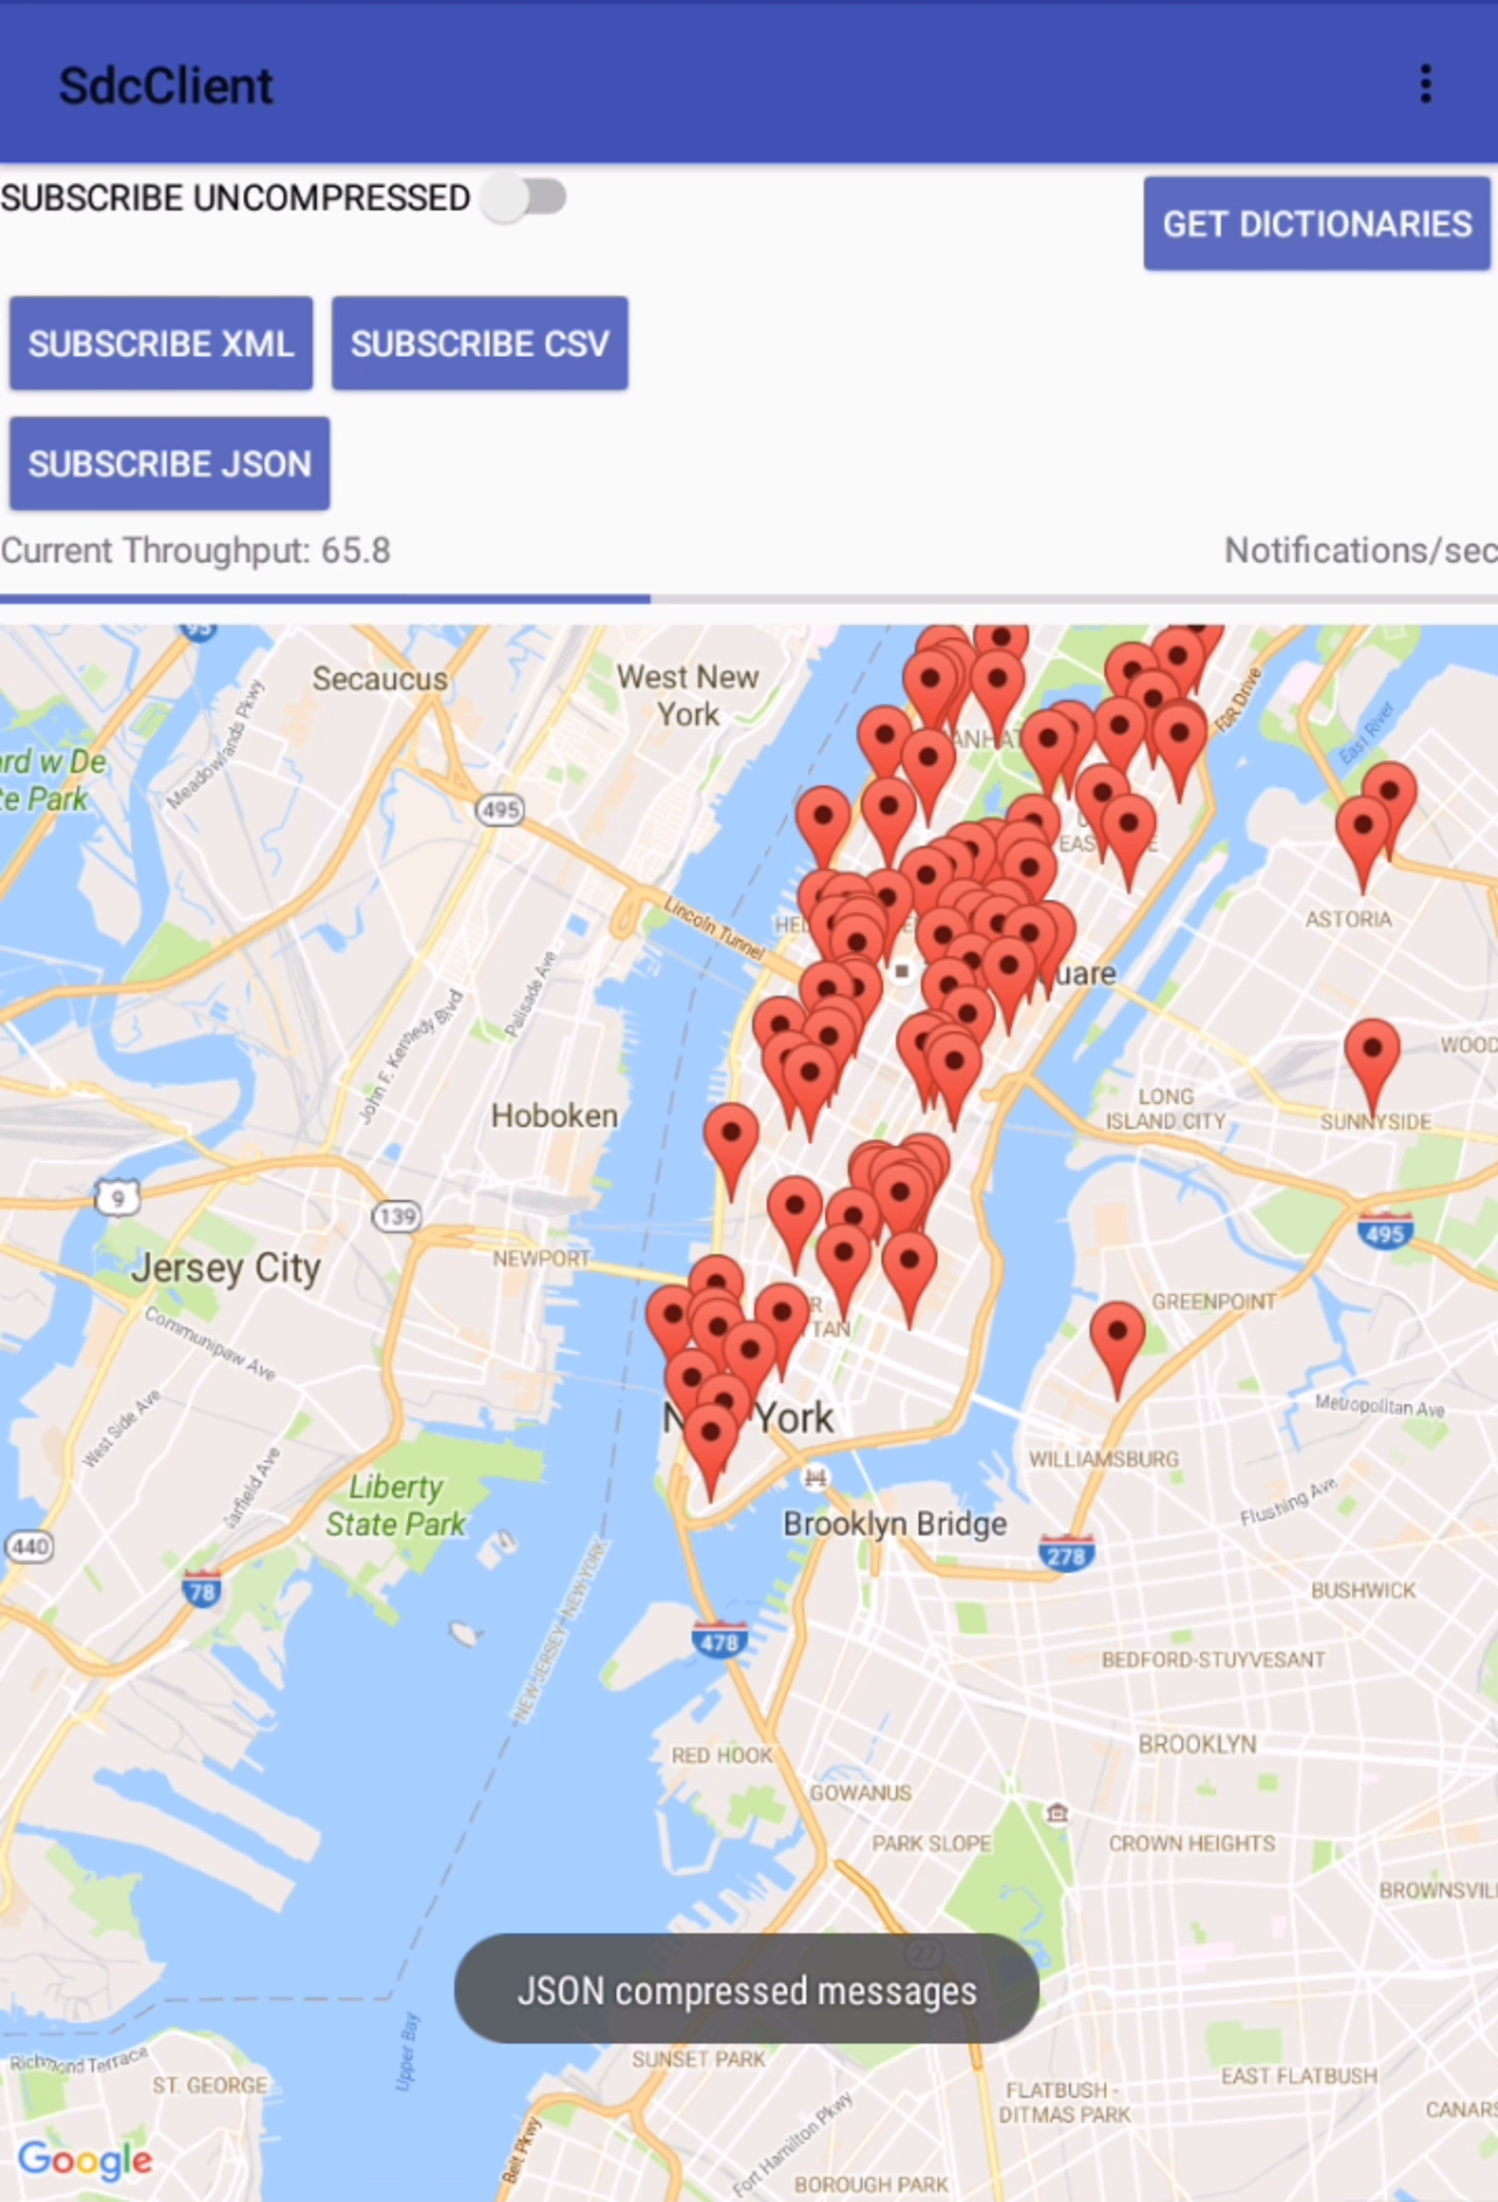
\includegraphics[scale=0.28]{json_c.pdf}
  \captionsetup{width=0.9\textwidth}
  \caption{JSON compressed notifications}
  \label{figures:json_c}
\end{minipage}
\end{figure}



%%%%%%%%csv%%%%%%%%%%%

\begin{figure}
\noindent\begin{minipage}{.5\textwidth}
  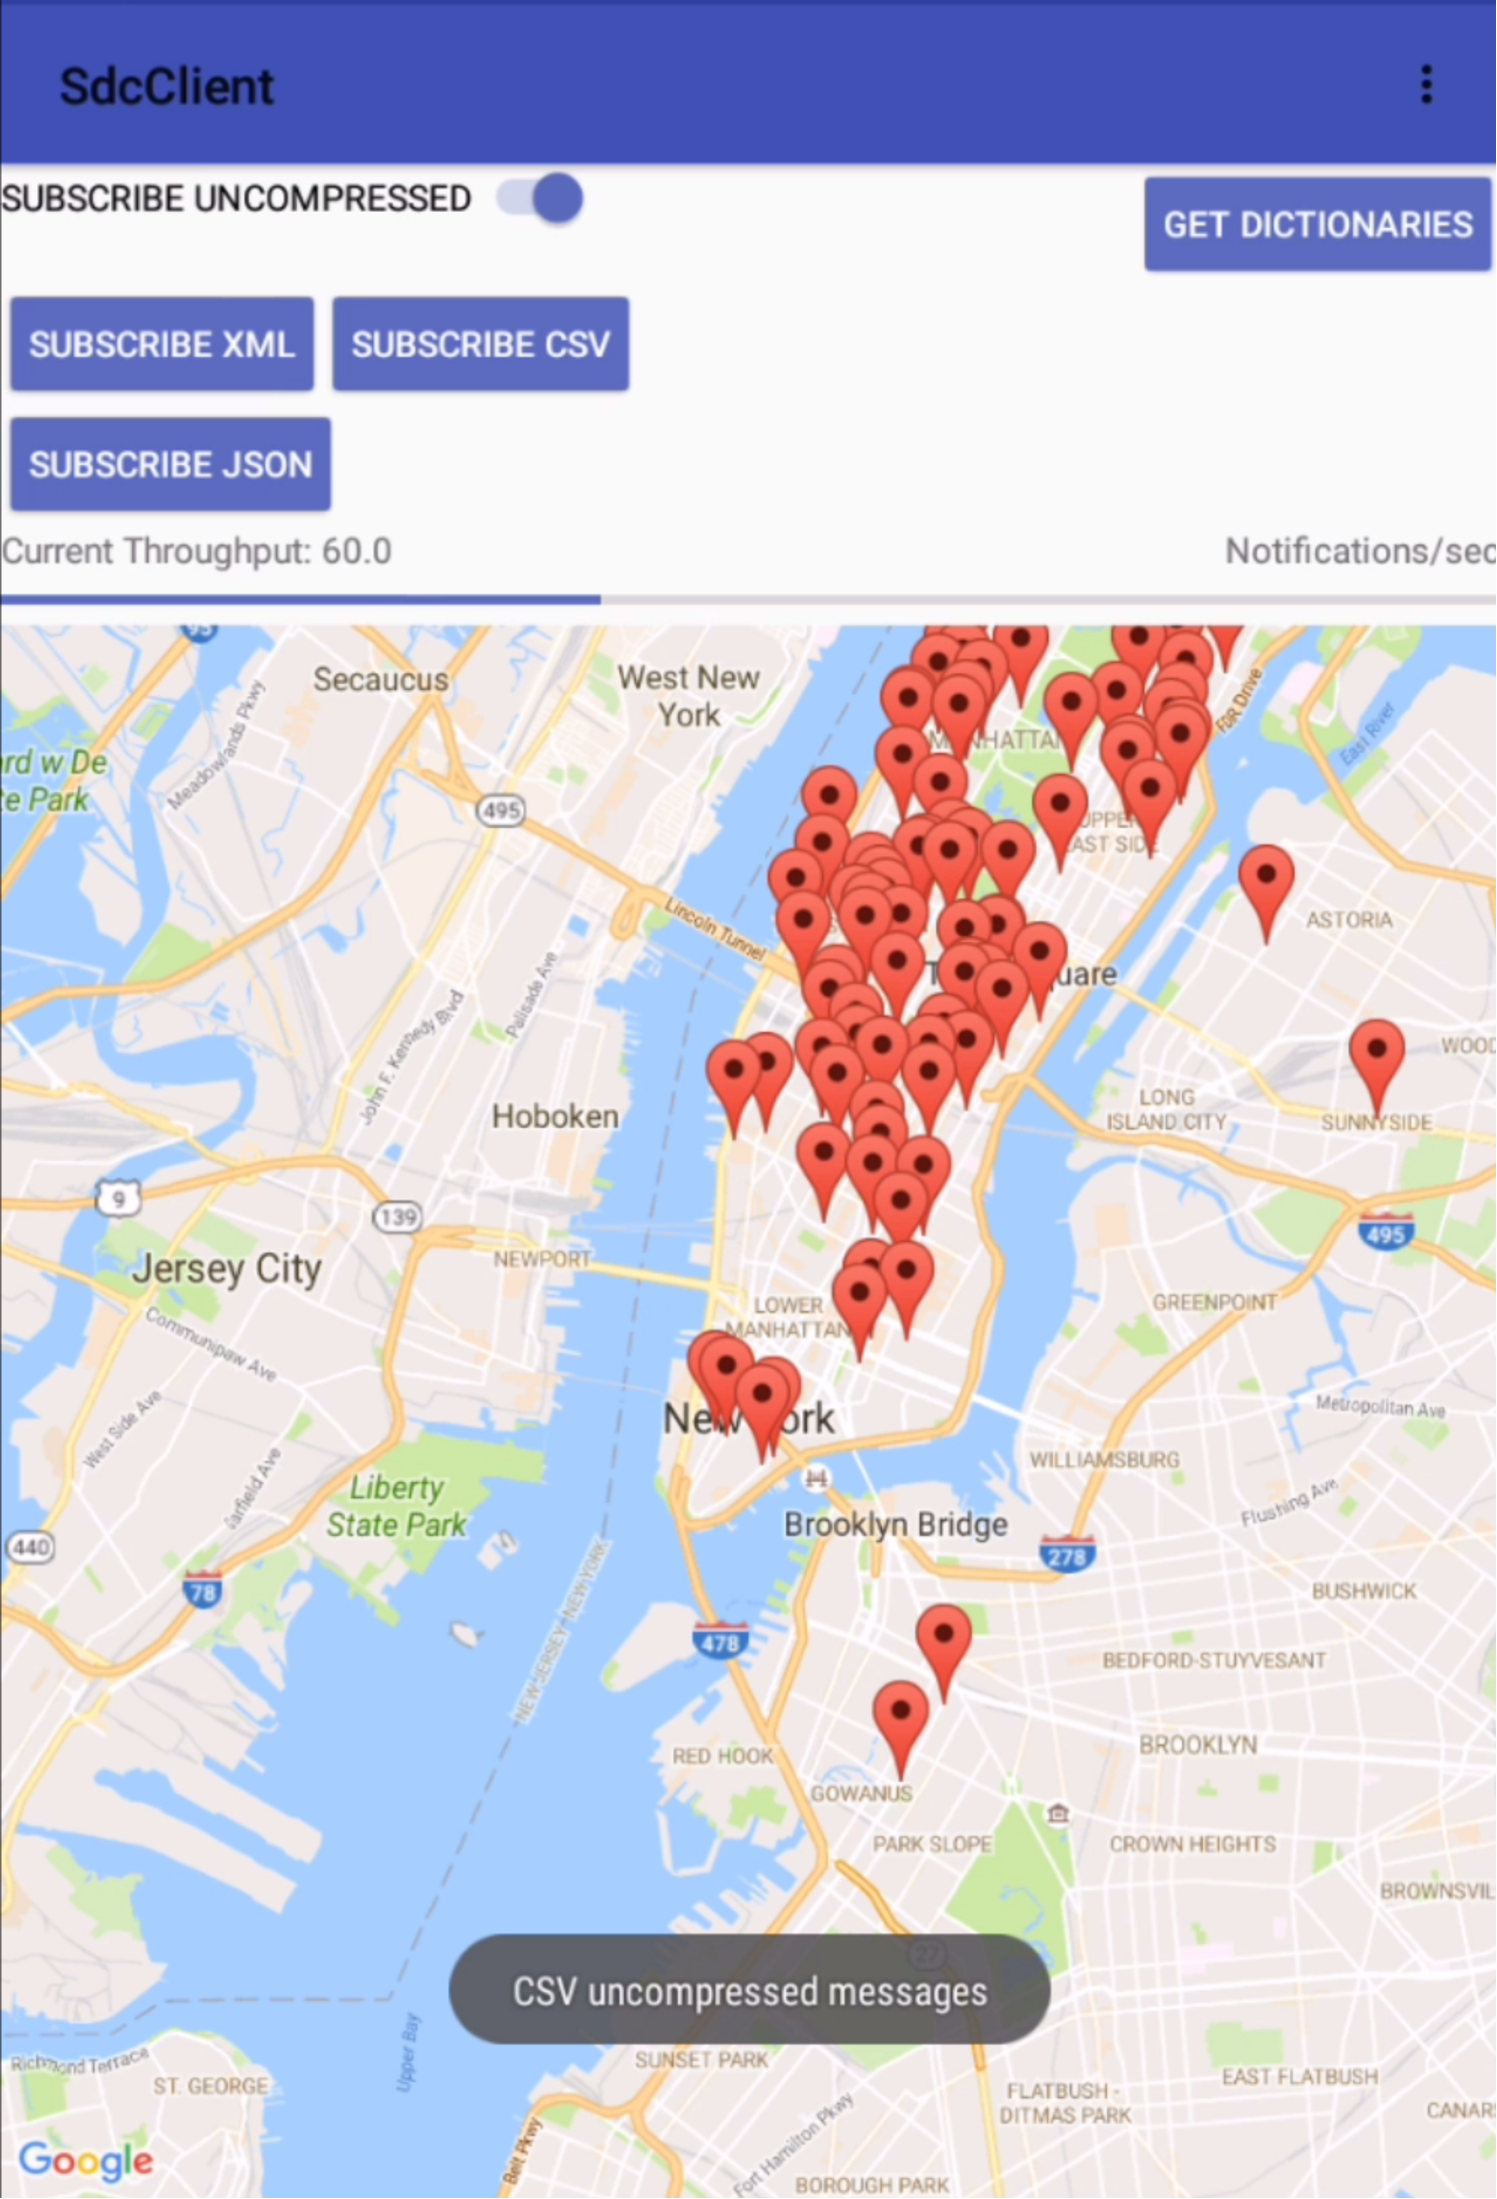
\includegraphics[scale=0.28]{csv_u.pdf}
  \captionsetup{width=0.9\textwidth}
  \caption{CSV uncompressed notifications}
  \label{figures:csv_u}
\end{minipage}%
\begin{minipage}{.5\textwidth}
  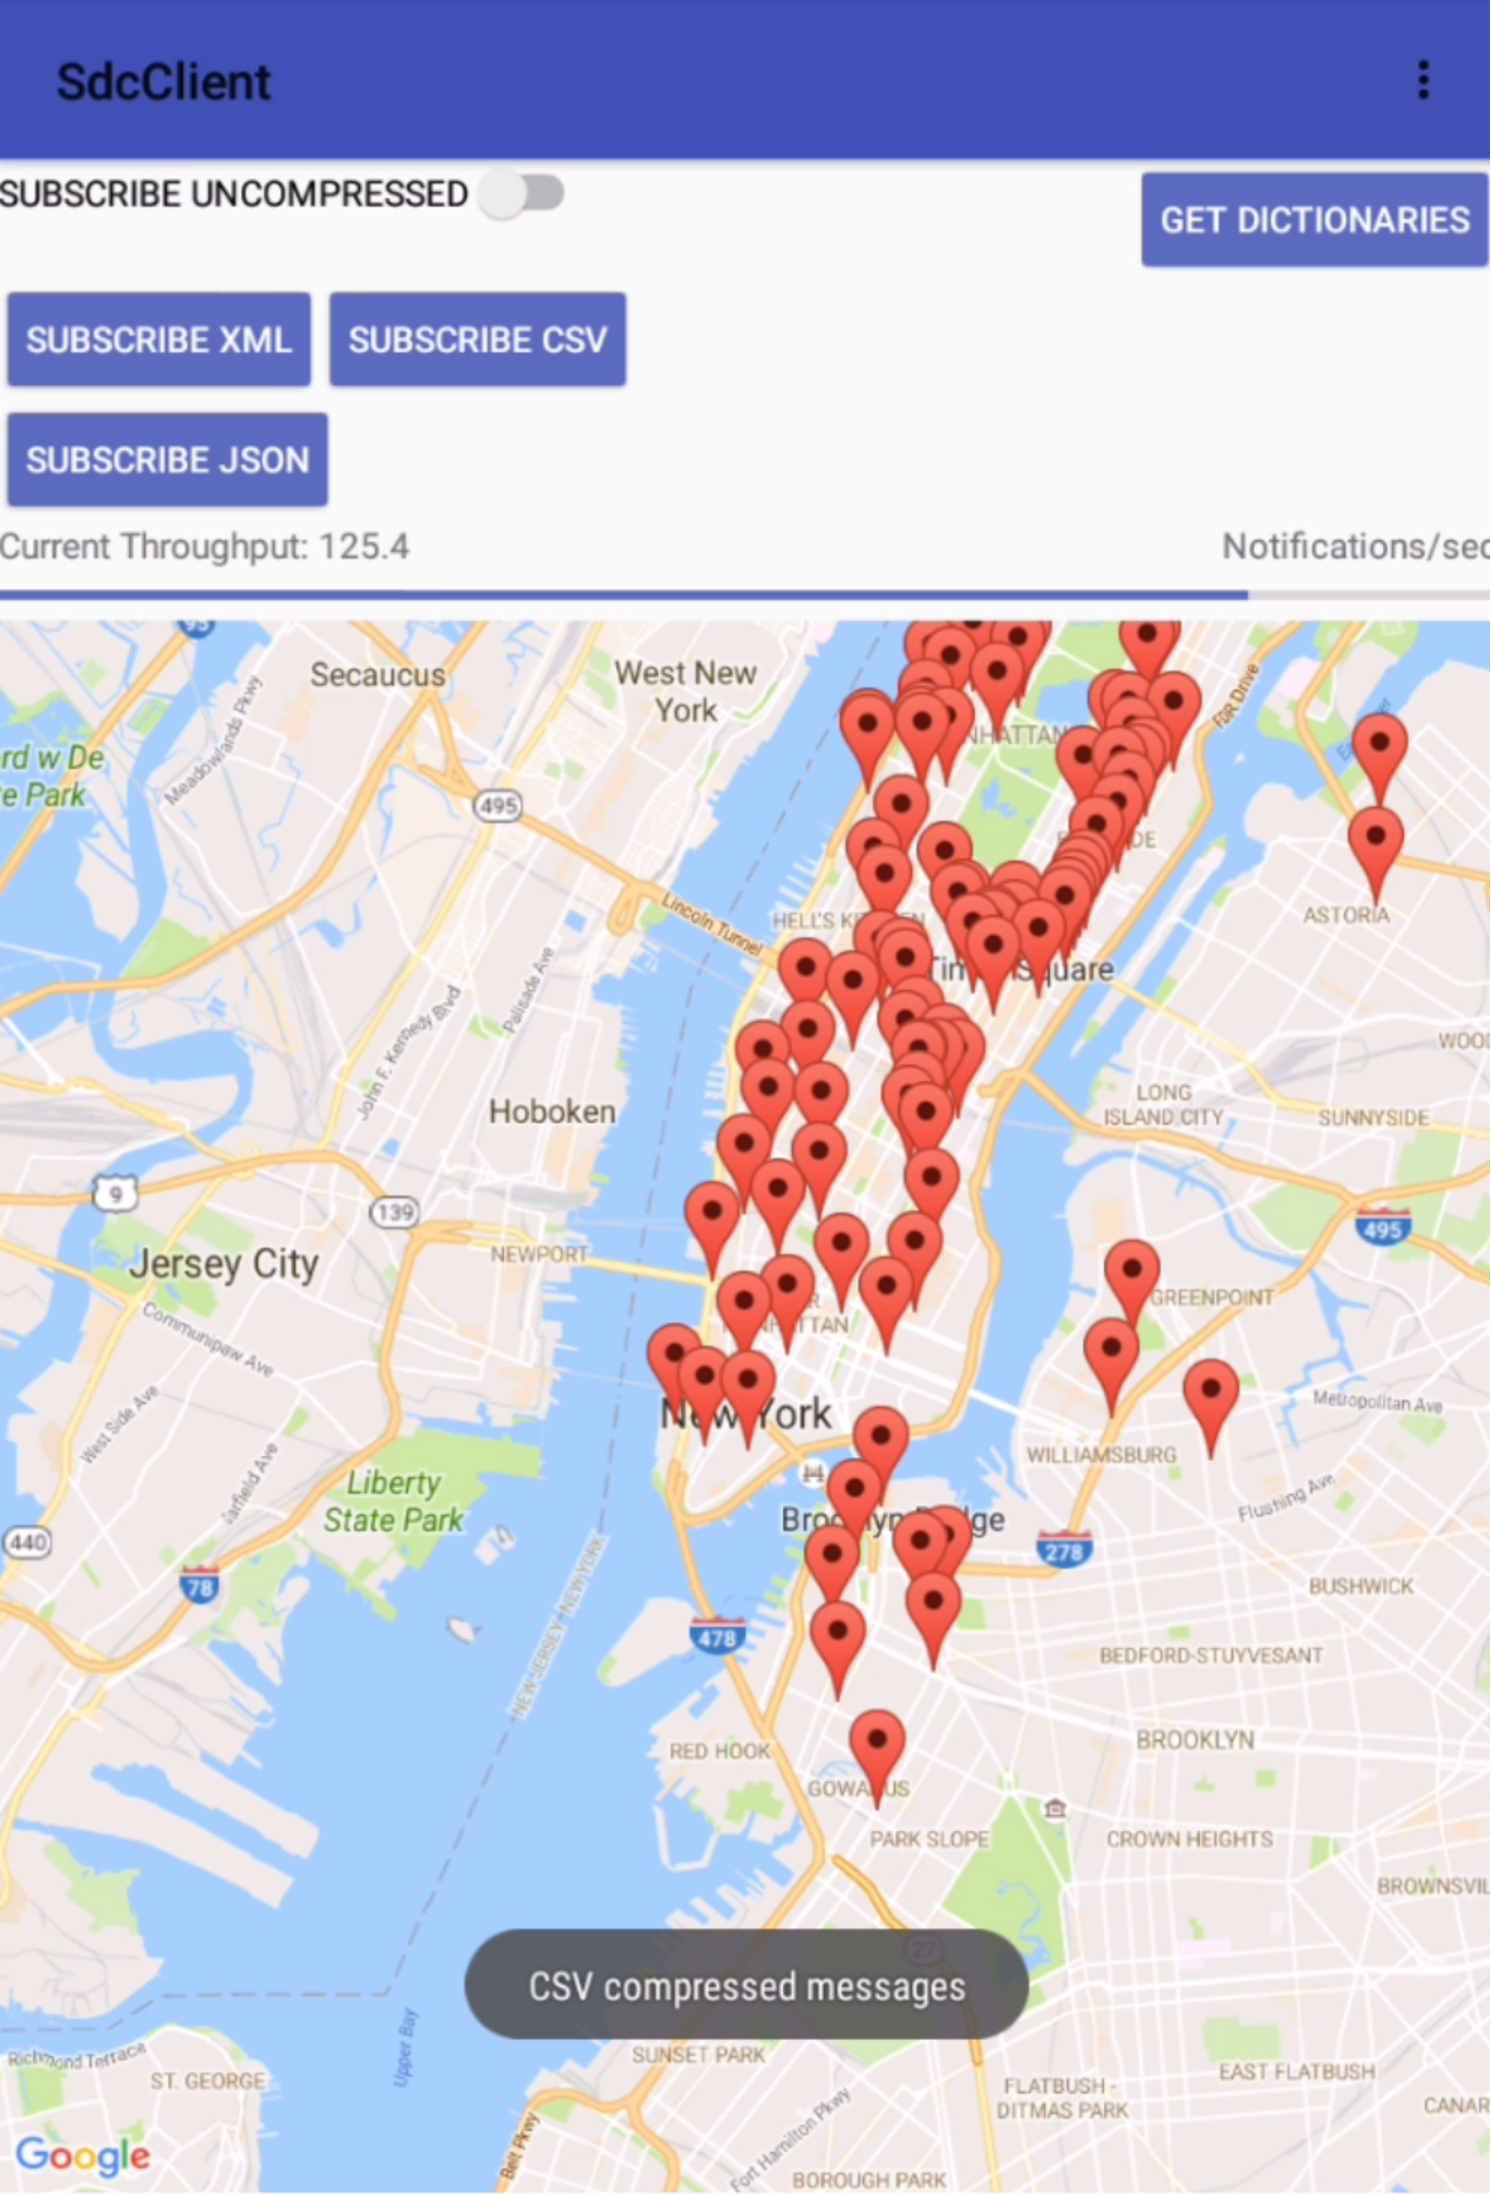
\includegraphics[scale=0.28]{csv_c.pdf}
  \captionsetup{width=0.9\textwidth}
  \caption{CSV compressed notifications}
  \label{figures:csv_c}
\end{minipage}
\end{figure}

